\documentclass[twoside,10pt]{article}
\usepackage{/Users/bradenhoagland/latex/styles/toggles}
%\toggletrue{sectionbreaks}
%\toggletrue{sectionheaders}
\newcommand{\docTitle}{Math 611 - HW 6}
\usepackage{/Users/bradenhoagland/latex/styles/common}
\importStyles{modern}{rainbow}{boxy}

%\renewcommand{\theenumi}{\alph{enumi}}

\begin{document}
%\tableofcontents

% ------------------------------
% 1.3: 16
% ------------------------------
\begin{exer}[1.3: 16]
	If $q:Y\to Z$ and $qp:X\to Z$ are covering maps (in the sense of Hatcher, i.e. not surjective), then so is $p:X\to Y$. It's normal if $qp:X\to Z$ is normal.
\end{exer}

\textbf{Covering map:} Let $y \in Y$, let $U_1$ be a neighborhood of $y$ that's evenly covered by $q$, and let $U_2$ be a neighborhood of $y$ evenly covered by $pq$. Then $U_1 \isct U_2$ is evenly covered by both. Since $Z$ is locally path connected, there is some $U \subset U_1 \isct U_2$ that's path connected and still evenly covered.

We know $q^{-1}(U) = \bigsqcup_{i \in \mathcal{J}} V_i$, where each $V_i \cong U$ via $q$. Let $V$ be the $V_i$ that contains $y$, then we claim that $V$ is evenly covered by $p$. First off, note that since $V \cong U$ and $U$ is path connected, so is $V$. Also note that $(qp)^{-1}(U) = \bigsqcup_{\alpha \in \mathcal{A}}W_{\alpha}$, where each $W_{\alpha}\cong U$ via $pq$ (and is thus path connected, too). We then know
\[
	p^{-1}(V) \subset p^{-1}(q^{-1}(U)) = (qp)^{-1}(U) = \bigsqcup_{\alpha \in \mathcal{A}}W_{\alpha}.
\] We now must show that $p^{-1}(V) = \bigsqcup_{\beta \in \mathcal{B}}W_\beta$ for $\mathcal{B} \subset \mathcal{A}$, but this ends up being a consequence of path connectedness. Suppose there's some $W_{\alpha}$ intersects more than one $p^{-1}(V_i)$, then we've disconnected that particular $W_\alpha$, a contradiction. Thus each $W_a$ lies inside of 1 and only 1 $p^{-1}(V_i)$. This implies that $p^{-1}(V) = \bigsqcup_{\beta \in \mathcal{B}}W_\beta$, as desired. This shows that $p$ is a covering map (in the sense of Hatcher, i.e. missing the surjectivity requirement).

\textbf{Normal:} Suppose $y \in Y$ and $x_0,x_1 \in p^{-1}(y)$, then we want to find some $\tau \in G(X)$ such that $\tau x_0 = x_1$. Now $x_0,x_1$ are both lifts of $q(y)$ under the covering map $qp$, and that covering map is normal, so there is some homeomorphism $\sigma:X\to X$ sending $x_0 \mapsto x_1$ and making the following commute.
\[
\begin{tikzcd}
	X \rar{\sigma}\dar["qp"'] & X \arrow[dl,"qp"] \\
	Z
\end{tikzcd}
\] 
We can now transform this deck transformation for $pq$ into one for $p$. Like any space, $X$ can be be partitioned into its path components, i.e. $X = \bigcup_{i} P_i$ for each $P_i$ the path component of $X$ containing $x_i$. We'll define $\tau$ in terms of these path components.

Since $\sigma$ is a homeomorphism, it must map path components onto path components, i.e. $\sigma: P_i \mapsto P_j$ In particular, we know $\sigma(P_0) = P_1$. Define $\tau|P_0 = \sigma|P_0$. If $P_0 = P_1$, then define $\tau|P_k = \id_{}$ for all $k \neq 0$. If $P_0 \neq P_1$, then define $\tau|P_1 = \sigma^{-1}|P_1$ and $\tau|P_k = \id_{}$ for all $k \neq 0,1$. With this definition, $\tau$ is bijective, both $\tau,\tau^{-1}$ are continuous, and $\tau$ maps $x_0\mapsto x_1$. All that's left to check is that the following diagram commutes.
\[
\begin{tikzcd}
        X \rar{\tau}\dar["p"'] & X \arrow[dl,"p"] \\
        Y
\end{tikzcd}
\]
Let $x \in P_0$, then there is a path $h$ from $x_0$ to $x$. The two paths $p\tau h$ and $p h$ in $Y$ both start at the same point, so by unique path lifting, $p \tau h = ph$. Thus $(p\tau)(x) = (p\tau h)(1) = (ph)(1) = p(x)$, so the diagram commutes in this case. The argument is similar if $x \in P_1$ instead. If $x \in P_k$ for $k \neq 0,1$, then the diagram definitely commutes since we defined $\tau$ to be the identity in this case. Thus $X\stackrel{p}{\to } Y$ is a normal covering map.

\newpage

% ------------------------------
% 1.3: 18
% ------------------------------
\begin{exer}[1.3: 18]
$X$ has an abelian covering space that covers all other abelian covers. It is unique up to isomorphism. Describe it explicitly for $X = S^{1}\vee S^{1}$ and $X = S^{1}\vee S^{1}\vee S^{1}$.
\end{exer}

Consider the covering $\tilde{X} \stackrel{p}{\to } X$ corresponding to the subgroup $G := [\pi_1(X),\pi_1(X)]$ of $\pi_1(X)$. We claim that it's the desired covering.

\textbf{Abelian:} (This section is essentially one big application of Proposition 1.39 from the textbook). Commutator subgroups are normal, so $G$ is normal, so $\tilde{X}$ is normal. Thus $G(\tilde{X}) \cong \pi_1(X) / G$, but modding a group by its commutator gives an abelian group, so $G(\tilde{X})$ is abelian. Thus $\tilde{X}$ is an abelian cover.

\textbf{Covers every other abelian cover:} Suppose $\tilde{Y} \stackrel{q}{\to } X$ is another abelian cover, i.e. $H := p_{*}(\pi_1(\tilde{Y}))$ is normal and $G(\tilde{Y})$ is abelian. Now
\[
	G(\tilde{Y}) \cong \pi_1(X)/H \text{ is abelian } \iff G \subset H
\] since $G$ is the smallest normal subgroup making its quotient with $\pi_1(X)$ abelian. This means
\[
	p_*(\pi_1(\tilde{X})) = G \subset H = q_*(\pi_1(\tilde{Y})),
\] so we can apply the lifting criterion to get the following commutative diagram.
\[
\begin{tikzcd}
	& \tilde{Y} \dar{q} \\
	\tilde{X} \arrow[ur, dashed, "\exists \; \phi"] \rar{p} & X
\end{tikzcd}
\] We claim that $\phi$ is a covering map. Fix $\tilde{y} \in \tilde{Y}$ and consider $x := q(\tilde{y})$. This has neighborhoods $U$ (evenly covered by $p$) and $V$ (evenly covered by $q$). Then $U \isct V$ is evenly covered by both. Now consider the unique set $W$ in $q^{-1}(U \isct V)$ containing $\tilde{y}$. We claim that this is an evenly covered neighborhood of $\tilde{y}$ (which would make $\tilde{X}$ a covering of $\tilde{Y}$).

Since the above diagram commutes, we know there is some subset of $\tilde{X}$ that $\phi$ maps to $W$. Since $p$ is a homeomorphism on each homeomorphic copy of $U \isct V$ inside $\tilde{X}$, we know $\phi = p q^{-1}$ on each copy as well, meaning that $\phi$ itself is a homeomorphism. Thus $\phi$ is a covering map that evenly covers $W$.

\textbf{Unique up to iso:} Suppose $\tilde{Z}$ is an abelian covering space with the same properties as $\tilde{X}$. By a similar argument as above, we have the following commutative diagram.
\[
\begin{tikzcd}
	& \tilde{Z} \arrow[dl, dashed, shift left, "\exists \;\psi"] \dar{q} \\
	\tilde{X} \arrow[ur, dashed, shift left, "\exists \;\phi"] \rar["p"'] & X
\end{tikzcd}
\] 
We claim that $\phi$ and $\psi$ are mutually inverse (and thus isomorphisms). Now consider the following diagram.
\[
\begin{tikzcd}
	& \tilde{X} \dar{p} \\
	\tilde{X} \arrow[ur, "\psi\phi"]\rar{p} & X
\end{tikzcd}
\] It commutes since $p \psi \phi = q \phi = p$. A possible lift of $p$ is $\id_{\tilde{X}}$, so by uniqueness of lifts, $\psi\phi = \id_{\tilde{X}}$. Using similar logic, we get $\phi \psi = \id_{\tilde{Z}}$. Thus $\phi$ and $\psi$ are isomorphisms.

\textbf{Examples:} When $X = S^{1}\vee S^{1}$, we have $\text{ab}(\pi_1(X)) \cong \text{ab}(\mathbb{Z} * \mathbb{Z}) \cong \mathbb{Z}^2$. Thus we need a covering space $\tilde{X} \stackrel{p}{\to } X$ with $p_{*}(\pi_1(\tilde{X})) = \mathbb{Z}^{2}$. Let $\tilde{X}$ be the lattice in $\R^{2}$ with squares as shown below.

\[
\begin{tikzcd}
	{} \arrow[r, "a"]                 & {}                \\
{} \arrow[r, "a"'] \arrow[u, "b"] & {} \arrow[u, "b"']
\end{tikzcd}
\] 

Note that $p_{*}$ maps $a \mapsto a$ and $b \mapsto b$, so $p_{*}(\pi_1(\tilde{X})) = p_*(\ang{a,b}) = \ang{a,b} \cong \mathbb{Z}^{2}$, as desired.

Similarly, when $X= S^{1}\vee S^{1}$, we have $\text{ab}(\pi_1(X)) \cong \mathbb{Z}^{3}$. Then we can use the lattice in $\R^{3}$ with cubes as shown below.

\[
\begin{tikzcd}
                                                  & {} \arrow[r, "a"]                                 & {}                \\
{} \arrow[r, "a"] \arrow[ru, "c"]                 & {} \arrow[ru, "c"] \arrow[u, "b"] \arrow[r, "a"'] & {} \arrow[u, "b"] \\
{} \arrow[r, "a"'] \arrow[u, "b"] \arrow[ru, "c"] & {} \arrow[u, "b"] \arrow[ru, "c"']                &                  
\end{tikzcd}
\] 


Again, we have $p_{*}(\pi_1(\tilde{X})) \cong \ang{a,b,c}\cong \mathbb{Z}^{3}$, as desired.

\newpage

% ------------------------------
% 1.3: 19
% ------------------------------
\begin{exer}[1.3: 19]
Use 1.3: 18 to show that a closed orientable surface $M_{g}$ has a connected normal covering space with deck transformation group isomorphic to $\mathbb{Z}^{n}$ iff $n \leq 2g$. For $n=3$ and $g \geq 3$, describe such a covering explicitly as a subspace of $\R^{3}$ with translations of $\R^{3}$ as deck transformations.
\end{exer}

\textbf{First part:} We know that the fundamental group of a closed genus $g$ surface is
\[
	\pi_1(M_{g}) \cong \ang{a_1, \dots, a_g, b_1, \dots, b_g \;|\; [a_1,b_1] \cdots [a_g,b_g] },
\] and its abelianization is
\[
	\text{ab}(\pi_1(M_{g})) \cong \ang{a_1, \dots, a_g, b_1, \dots, b_g} \cong \mathbb{Z}^{2g}.
\] 

We also know that if $\tilde{X}$ is a normal covering space of $\tilde{X}$, then $G(\tilde{X}) \cong \pi_1(X) / H$, where is the subgroup of $\pi_1(X)$ corresponding to $\tilde{X}$. Now by the previous exercise, we know $M_g$ has an abelian covering space $\tilde{X}$ that covers all others, and we showed that it corresponds to $H = \left[ \pi_1(M_g), \pi_1(M_g) \right]$. Its deck transformation group is then $\text{ab}(\pi_1(M_g)) \cong \mathbb{Z}^{2g}$.

The subgroups of $\mathbb{Z}^{2g}$ are exactly the $\mathbb{Z}^n$ for $n \leq 2g$, i.e. for all $n \leq 2g$, there exist $G_n$ such that
\[
	\frac{\pi_1(M_g)}{\left[ \pi_1(M_g), \pi_1(M_g) \right]} / \frac{G_n}{\left[ \pi_1(M_g), \pi_1(M_g) \right]} \cong \frac{\pi_1(M_g)}{G_n} \cong \mathbb{Z}^{n}.
\] Then the deck transformation group of the covering space corresponding to $G_n$ is $\mathbb{Z}^{n}$. Since there are no other subgroups of $\mathbb{Z}^{2g}$, these are no other coverings with this form of deck transformation group.

\newpage
\textbf{Covering in $\R^{3}$:} In 3 dimensions we can take the integer lattice in $\R^{3}$ (as in the previous problem), widen each line, and make each tube hollow to get a lattice with elements as below.

\vspace{2in}

Each of the three ``axes" pictured above in the tube corresponds to the three main loops in $M_3$.

\vspace{2in}

Thus every copy of this figure in the lattice is itself a covering of $M_3$, so the whole lattice is as well. The deck transformations of this lattice are the translations
\begin{align*}
	x+1, y, z; \\
	x, y+1, z; \\
	x, y, z+1.
\end{align*}
Thus the deck transformation group is given by $\mathbb{Z}^{3}$, as desired.

\newpage

% ------------------------------
% 1.3: 20
% ------------------------------
\begin{exer}[1.3: 20]
Construct nonnormal covering spaces of the Klein bottle by a Klein bottle and by a torus.
\end{exer}

\textbf{Cover with Klein bottle:} Consider the following covering map $ p:K\to K$, where $K$ is the Klein bottle. We divide $K$ into three identical parts and map each part onto $K$ in the natural way.

\begin{figure}[H]
	\centering
	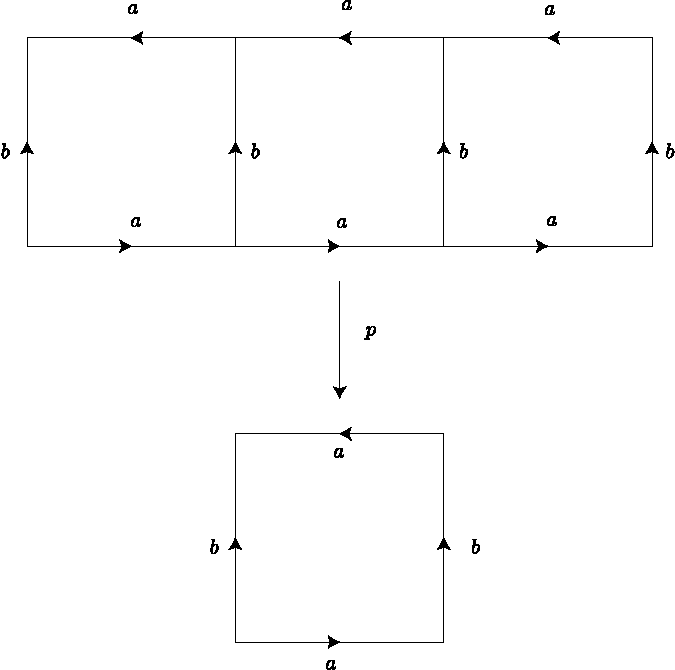
\includegraphics[scale=1]{fig/20a.pdf}
	%\caption{}
\end{figure}

The induced map $p_{*}$ then maps $a \mapsto a^{3}$ and $b \mapsto b^{2}$. Since we know by van Kampen that
\[
	\pi_1(K) \cong \ang{a,b \;|\; abab^{-1}},
\] this means
\[
	H := p_*(\pi_1(K)) \cong \ang{a^{2},b \;|\; abab^{-1}}.
\] We claim that this is not a normal subgroup of $\pi_1(K)$. Consider $g = a \in \pi_1(K)$ and $n = b \in H$. If $H$ is normal in $\pi_1(K)$, then
\[
g n g^{-1} = a b a^{-1} = a^{2}b \in H,
\] where the last equality follows from the relation in $H$. But this isn't true since $a^{2}$ cannot be generated by $a^{3}$ and $b$. Thus $H$ is not normal in $\pi_1(K)$, so the covering space is not normal.

\textbf{Cover with torus:} Consider the following covering map $q:T^{2}\to K$. We divide the torus $T^{2}$ into two separate compartments, then map onto $K$ in the obvious way for each compartment.

\begin{figure}[H]
	\centering
	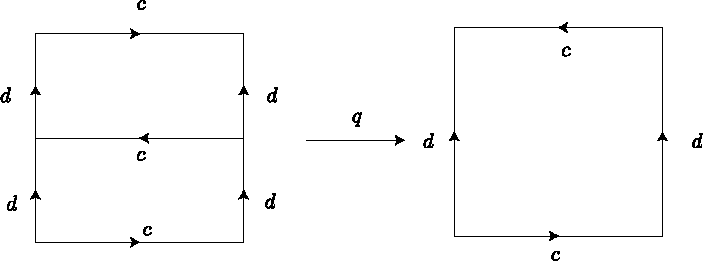
\includegraphics[scale=1]{fig/20b.pdf}
	%\caption{}
\end{figure}

Note that $q_*$ maps $c \mapsto a$ and $d \mapsto b^2$. Now consider the subgroup of $\pi_1(T^{2})$ generated by $c^{3}$ and $c^{2}d$. This corresponds to a covering of the torus by itself $p:T^{2}\to T^{2}$. This covering is pictured below, where we send each horizontal component of the boundary to $c$ and we send each vertical component to $c^{2}d$ (essentially looping it around the other circle composing $T^{2}$ twice before sending it to the natural place).

\begin{figure}[H]
	\centering
	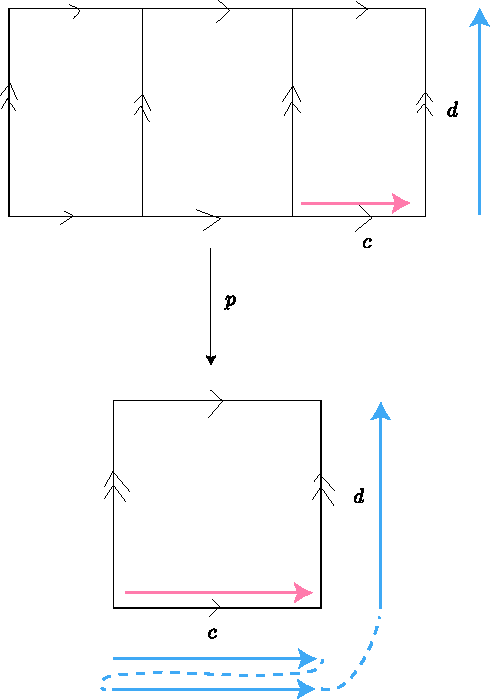
\includegraphics[scale=0.8]{fig/20c.pdf}
	%\caption{}
\end{figure}

Then the composition $qp:T^{2}\to K$ is a covering of the Klein bottle by a torus such that $(qp)_{*}$ maps $c \mapsto a^{3}$ and $d \mapsto a^{2} b^2$. By a similar argument as above, though, $a b a^{-1} = a^{2}b$ is not in this subgroup, so it is not normal and thus the covering is not normal.

\newpage

\end{document}
